\title{Web-Based Supporting Materials for\\
	``RNN-Based Counterfactual Prediction'' by Jason Poulos}

\date{}

%%%%%%%%%%%%%%%%%%%%%%%%%%%%%%%%%%%%%%%%%%%%%%%%%%
% Set document class
\documentclass[12pt]{article}

% Define packages
\usepackage{hyperref, url} 
\usepackage{graphicx,amsfonts,psfrag,layout,subcaption,array,longtable,lscape,booktabs,dcolumn,amsmath,amssymb,amssymb,amsthm,setspace,epigraph,chronology,color,colortbl,caption,wasysym,diagbox,natbib,colortbl}
\usepackage[]{graphicx}\usepackage[]{color}
\usepackage[page]{appendix}
\usepackage[section]{placeins}
\usepackage[linewidth=1pt]{mdframed}
\usepackage[margin={1in}]{geometry} %1 inch margins

%% Reference labels in the online appendix
\usepackage{xr}
\externaldocument{rnns-causal}

% Footnotes stick at the bottom
\usepackage[bottom]{footmisc}

% Caption keys
\usepackage{mathtools,tikz,caption}
\captionsetup{labelfont=sc,labelsep=period}
\DeclareRobustCommand\sampleline[1]{%
	\tikz\draw[#1] (0,0) (0,\the\dimexpr\fontdimen22\textfont2\relax)
	-- (2em,\the\dimexpr\fontdimen22\textfont2\relax);%
}

\usetikzlibrary{plotmarks}

% Wes Anderson colors

\usepackage{xcolor}

\definecolor{Darjeeling11}{HTML}{FF0000}
\definecolor{Darjeeling15}{HTML}{5BBCD6}

% New footnote characters
\usepackage{footmisc}
\DefineFNsymbols{mySymbols}{{\ensuremath\dagger}{\ensuremath\ddagger}\S\P
	*{**}{\ensuremath{\dagger\dagger}}{\ensuremath{\ddagger\ddagger}}}
\setfnsymbol{mySymbols}

% New tabular environment
\usepackage{tabularx}
\newcolumntype{Y}{>{\raggedleft\arraybackslash}X}% raggedleft column X

% Define appendix 
\renewcommand*\appendixpagename{Appendix}
\renewcommand*\appendixtocname{Appendix}

% Position floats
\renewcommand{\textfraction}{0.05}
\renewcommand{\topfraction}{0.95}
\renewcommand{\bottomfraction}{0.95}
\renewcommand{\floatpagefraction}{0.35}
\setcounter{totalnumber}{5}

% Colors for highlighting tables
\definecolor{Gray}{gray}{0.9}

% Different font in captions
\newcommand{\captionfonts}{\normalsize}

\makeatletter  % Allow the use of @ in command names
\long\def\@makecaption#1#2{%
	\vskip\abovecaptionskip
	\sbox\@tempboxa{{\captionfonts #1: #2}}%
	\ifdim \wd\@tempboxa >\hsize
	{\captionfonts #1: #2\par}
	\else
	\hbox to\hsize{\hfil\box\@tempboxa\hfil}%
	\fi
	\vskip\belowcaptionskip}
%\makeatother   % Cancel the effect of \makeatletter

% Set Spacing
%\singlespacing
%\doublespacing

% Number assumptions
\newtheorem*{assumption*}{\assumptionnumber}
\providecommand{\assumptionnumber}{}
\makeatletter
\newenvironment{assumption}[2]
{%
	\renewcommand{\assumptionnumber}{Assumption #1}%
	\begin{assumption*}%
		\protected@edef\@currentlabel{#1}%
	}
	{%
	\end{assumption*}
}
\makeatother

% Macros
\newcommand{\Adv}{{\mathbf{Adv}}}       
\newcommand{\prp}{{\mathrm{prp}}}                  % How to define new commands 
\newcommand{\calK}{{\cal K}}
\newcommand{\outputs}{{\Rightarrow}}                
\newcommand{\getsr}{{\:\stackrel{{\scriptscriptstyle\hspace{0.2em}\$}}{\leftarrow}\:}}
\newcommand{\andthen}{{\::\;\;}}    %  \: \; for thinspace, medspace, thickspace
\newcommand{\Rand}[1]{{\mathrm{Rand}[{#1}]}}       % A command with one argument
\newcommand{\Perm}[1]{{\mathrm{Perm}[{#1}]}}       
\newcommand{\Randd}[2]{{\mathrm{Rand}[{#1},{#2}]}} % and with two arguments
\newcommand{\E}{\mathrm{E}}
\newcommand{\Var}{\mathrm{Var}}
\newcommand{\Cov}{\mathrm{Cov}}
\DeclareMathOperator*{\plim}{plim}
\newcommand\independent{\protect\mathpalette{\protect\independenT}{\perp}}
\def\independenT#1#2{\mathrel{\rlap{$#1#2$}\mkern2mu{#1#2}}}
\newcommand{\possessivecite}[1]{\citeauthor{#1}'s [\citeyear{#1}]} 

\renewcommand*\contentsname{Table of contents}

%%%%%%%%%%%%%%%%%%%%%%%%%%%%%%%%%%%%%%%%%%%%%%%%%%%%%%%%%%%%%%%%%%%%%%%%%%%%

\begin{document}

\begin{singlespacing}
\maketitle \thispagestyle{empty}
\tableofcontents \thispagestyle{empty}
\end{singlespacing}

\pagenumbering{roman}% Roman-numbered pages (start from i)

\pagebreak
\pagenumbering{arabic}% Arabic-numbered pages (start from 1)

\section{Descriptive statistics}


\begin{figure*}[htbp]
	\centering
	\begin{subfigure}[t]{0.45\textwidth}
		\centering
		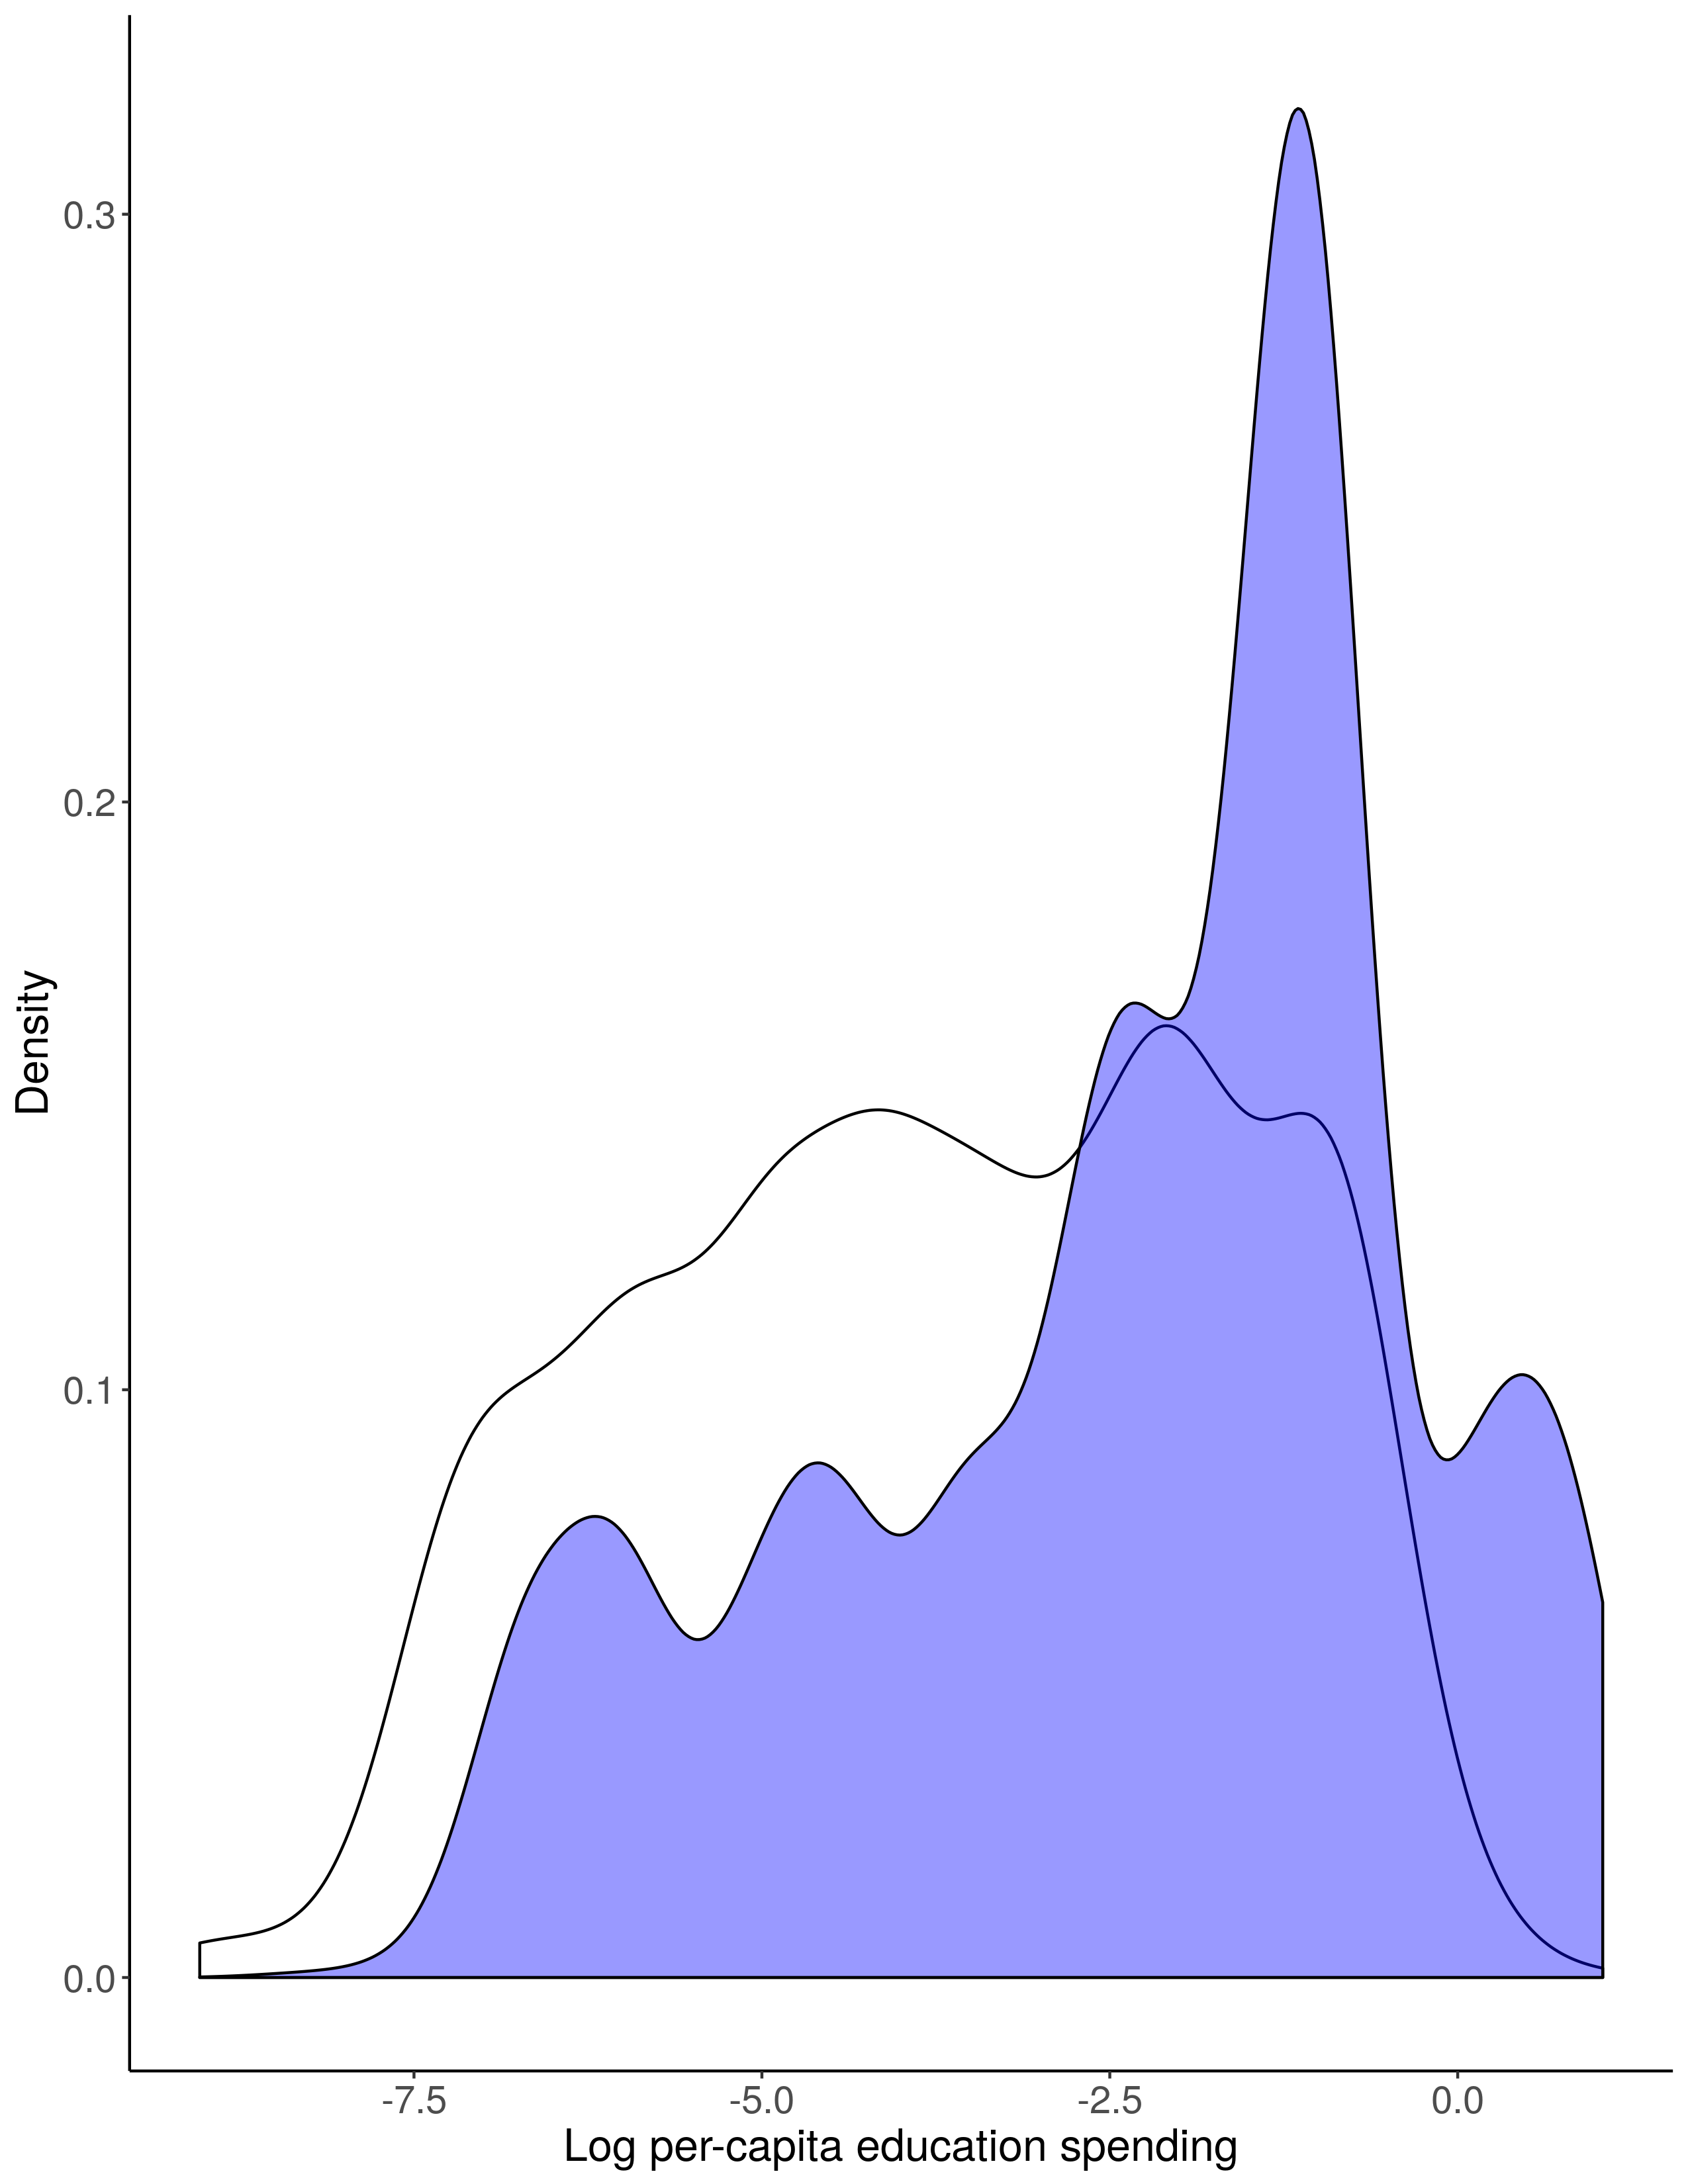
\includegraphics[width=\textwidth]{/media/jason/Dropbox/github/rnns-causal/results/plots/educ-dens.png}
		\caption{Unweighted \label{educ-dense}} 
	\end{subfigure}
	~ 
	\begin{subfigure}[t]{0.45\textwidth}
		\centering
		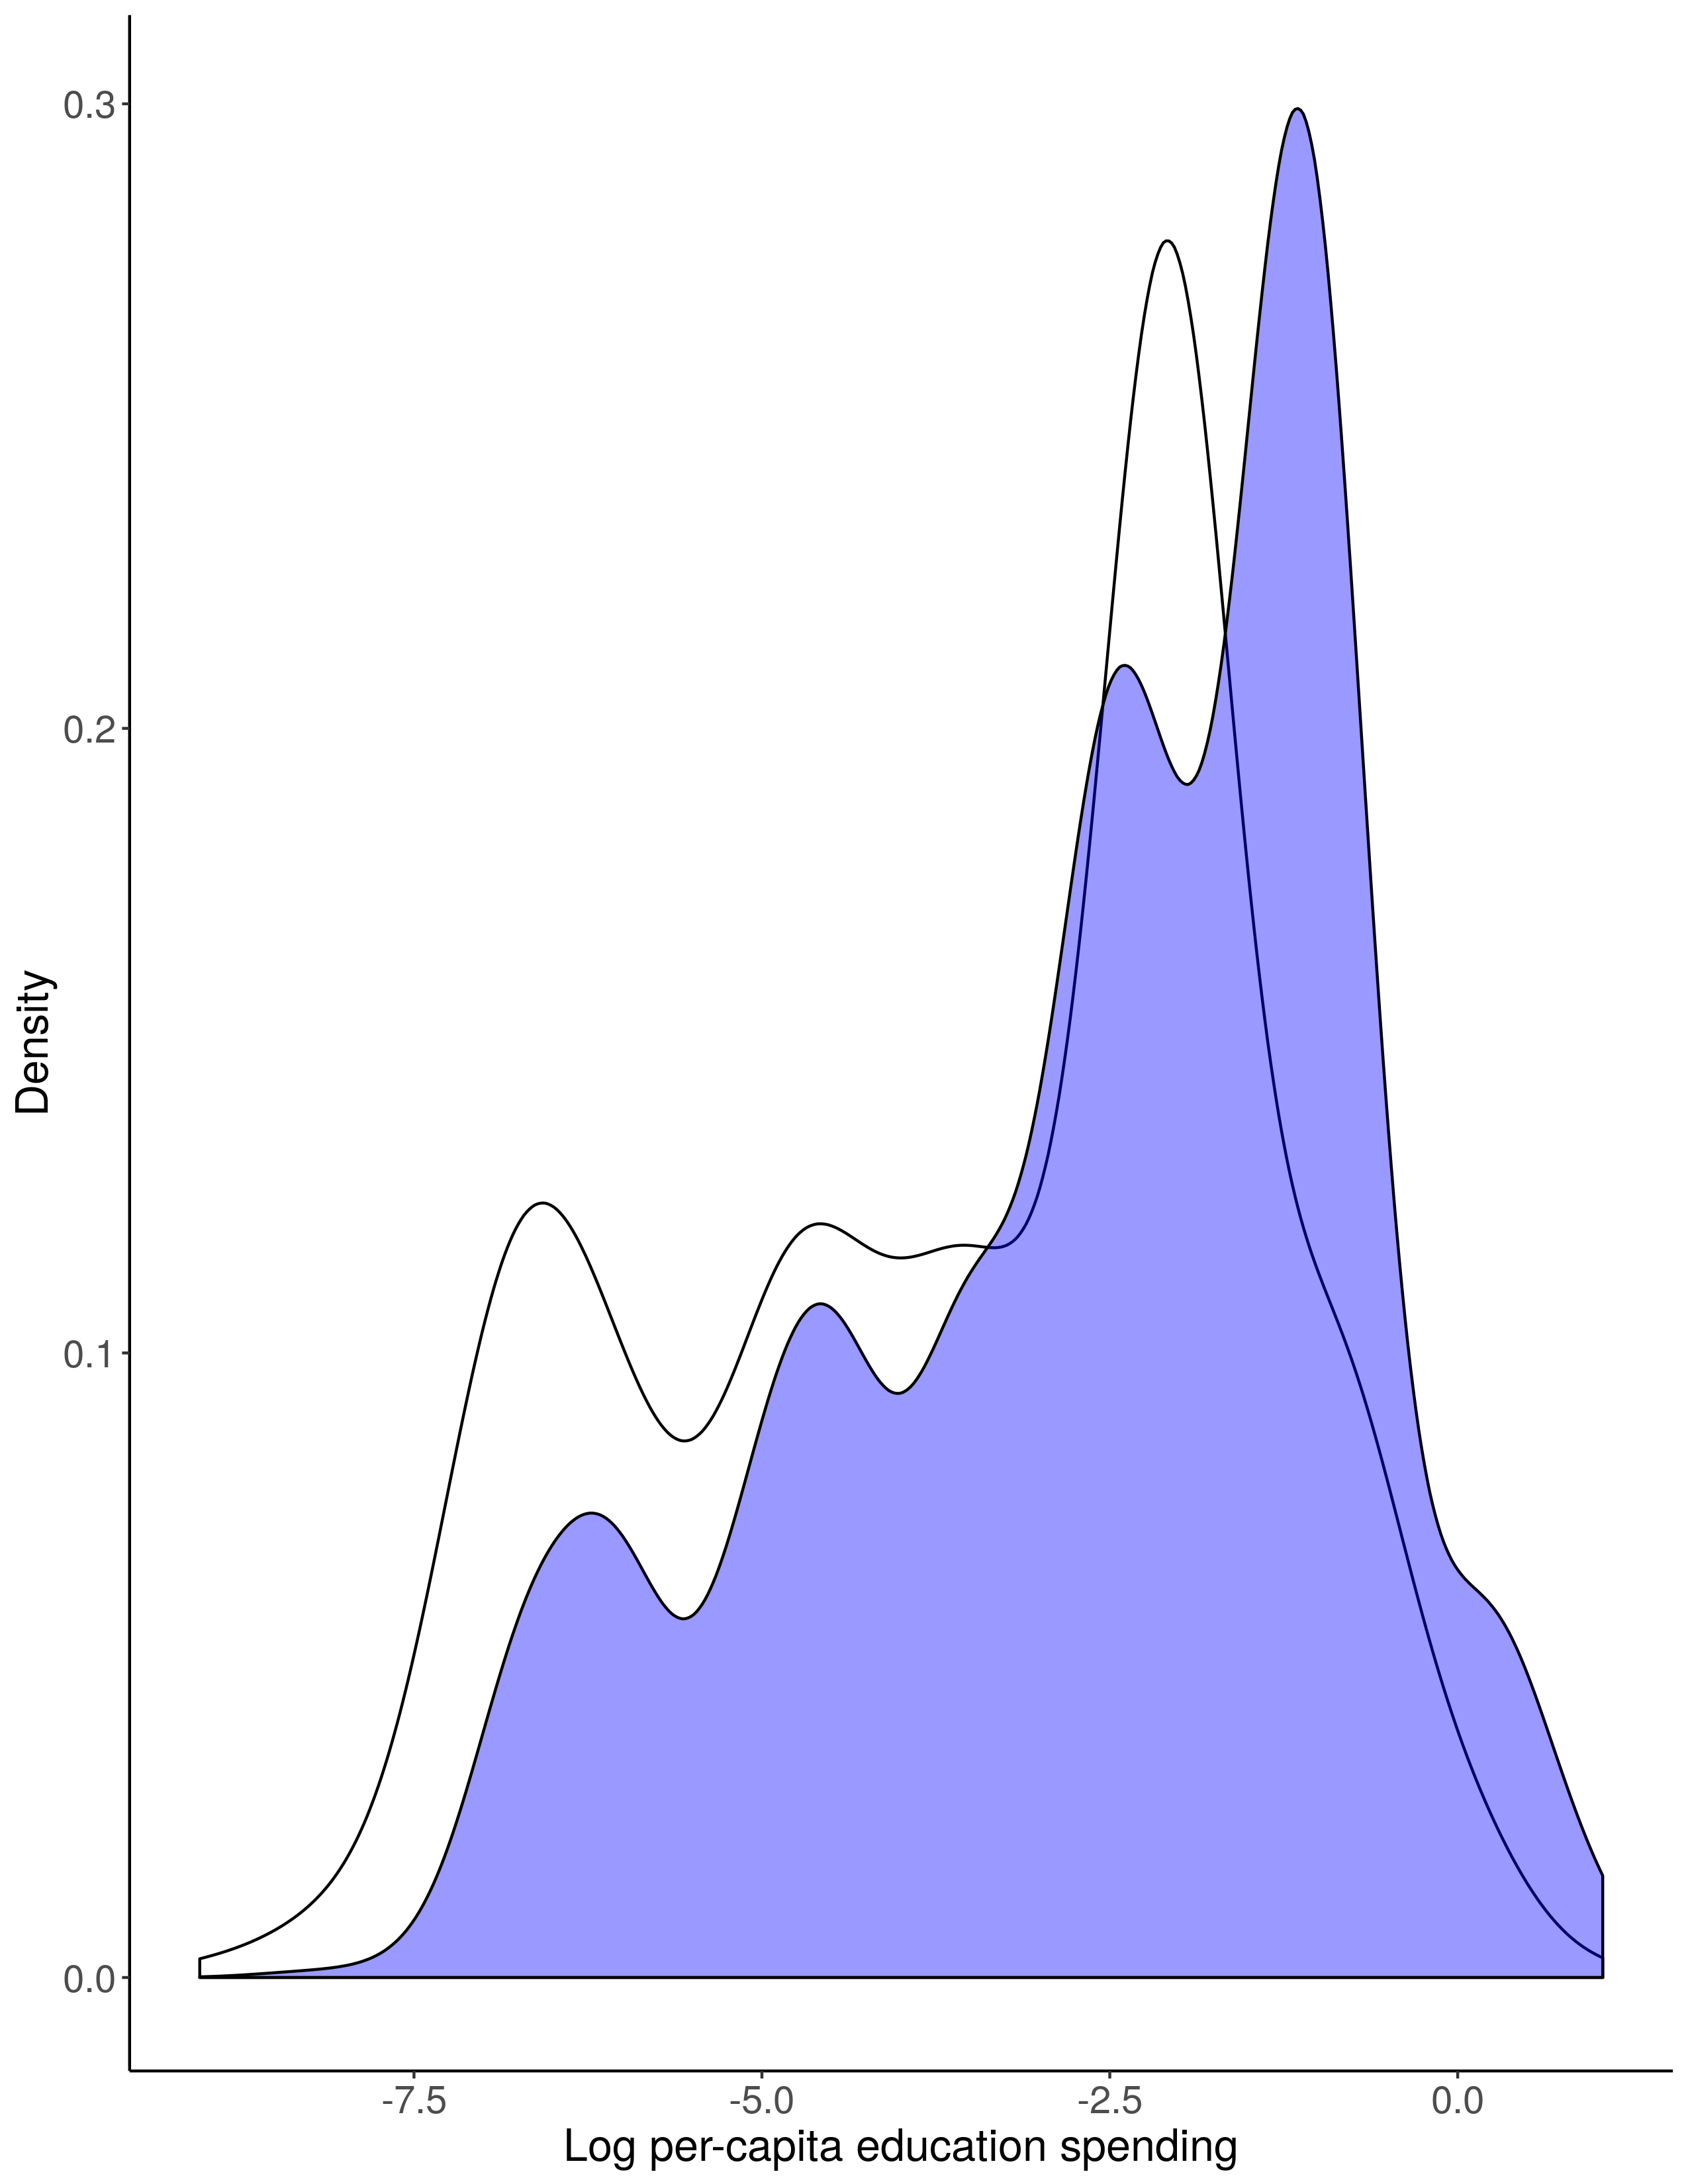
\includegraphics[width=\textwidth]{/media/jason/Dropbox/github/rnns-causal/results/plots/educ-dens-w.png}
		\caption{Weighted\label{educ-dense-w}}
	\end{subfigure}
	\caption{Pre-period densities of log per-capita state government education spending by treatment status. Density in \ref{educ-dense-w} weighted by propensity score.} 
\end{figure*}


\section{Estimates on education spending data}

\begin{figure*}[htbp]
	\centering
	\begin{subfigure}[t]{0.8\textwidth}
		\centering
		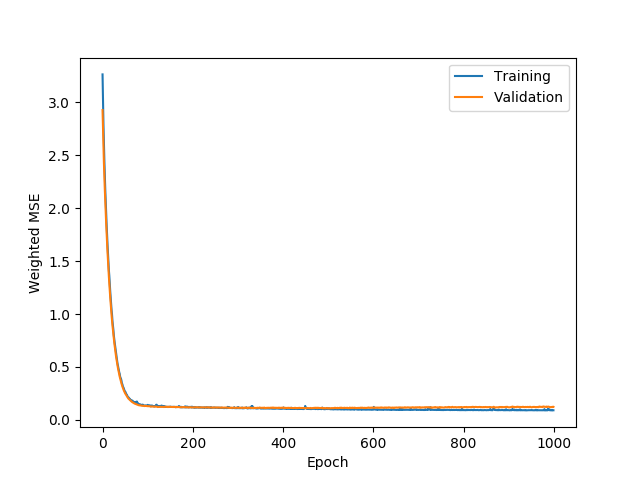
\includegraphics[width=\textwidth]{/media/jason/Dropbox/github/rnns-causal/results/plots/educ-ed-loss.png}
		\caption{Encoder-decoder networks} 
	\end{subfigure}
	~ 
	\begin{subfigure}[t]{0.8\textwidth}
		\centering
		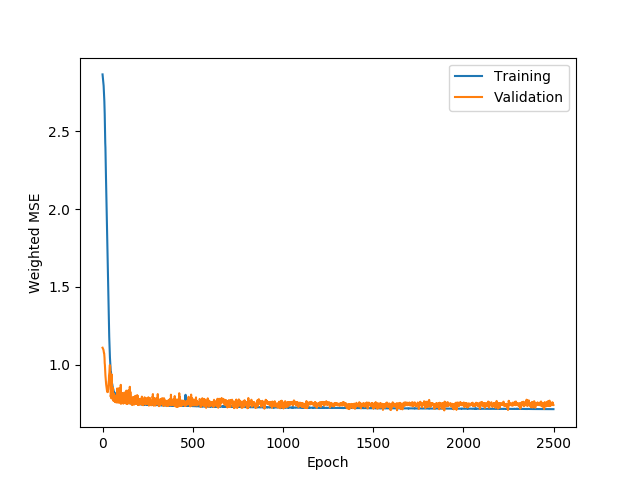
\includegraphics[width=\textwidth]{/media/jason/Dropbox/github/rnns-causal/results/plots/educ-rvae-loss.png}
		\caption{RVAE}
	\end{subfigure}
	\caption{RNNs training and validation loss on education spending data. \label{educ-loss}} 
\end{figure*}

\begin{figure*}[htbp]
	\centering
	\includegraphics[width=\textwidth]{/media/jason/Dropbox/github/land-reform/results/plots/encoder-decoder-plot-west-educpc.png}
	\caption{Observed (solid line) and counterfactual predicted (dashed line) outcomes for treated unit. Dashed vertical line represents intervention year. \label{state-capacity-plot}}
\end{figure*}

\begin{figure*}[htbp]
		\centering
		\includegraphics[width=\textwidth]{/media/jason/Dropbox/github/land-reform/results/plots/encoder-decoder-plot-effects-west-educpc.png}
		\caption{Time-series of post-period treatment effects in state capacity datasets. Darker line represents the effect on the actual treated unit and each lighter line represents the effects on placebo treated units. Shaded regions represent 95\% randomization confidence intervals. \label{state-capacity-plot-effects}}
\end{figure*}

\begin{table}[htbp]
	\begin{center}
		\caption{Encoder-decoder FPR and MSPE on state capacity placebo tests.\label{encoder-decoder-mpse}}
		\resizebox{\width}{!}{\input{/media/jason/Dropbox/github/land-reform/unsourced-paper/encoder-decoder-mpse}} \\
		\footnotesize{Note: Errors represent $\pm$ one standard deviation from the MSPE.}
	\end{center}
\end{table}

\begin{table}[htbp]
	\begin{center}
		\caption{LSTM FPR and MSPE on state capacity placebo tests.\label{lstm-mpse}}
		\resizebox{\width}{!}{\input{/media/jason/Dropbox/github/land-reform/unsourced-paper/lstm-mpse}} \\
		\footnotesize{Note: Errors represent $\pm$ one standard deviation from the MSPE.}
	\end{center}
\end{table}

\begin{figure*}[htbp]
		\centering
		\includegraphics[width=\textwidth]{/media/jason/Dropbox/github/land-reform/results/plots/encoder-decoder-plot-pvalues-west-educpc.png}
	\caption{Encoder-decoder networks: Per-period randomization $p$-values corresponding to treatment effects on treated and control units in state capacity datasets. Darker dot represents $p$-values associated with treatment effects on the actual treated unit and lighter dots represent $p$-values associated with the effects on control units \label{state-capacity-plot-pvalues}}
\end{figure*}

\itemize
\end{document}
